\chapter{HIỆN THỰC HỆ THỐNG PHÁT HIỆN TIN NÓNG}
\ifpdf
    \graphicspath{{Chapter3/Chapter3Figs/PNG/}{Chapter3/Chapter3Figs/PDF/}{Chapter3/Chapter3Figs/}}
\else
    \graphicspath{{Chapter3/Chapter3Figs/EPS/}{Chapter3/Chapter3Figs/}}
\fi

\section{Mở đầu}
Chương này sẽ trình bày về thiết kế, chi tiết cài đặt, các thư viện và framework được sử dụng để xây dựng hệ thống lọc rác tin tức.

\section{Mô hình hệ thống}
Dưới đây là mô hình của các thành phần chính hệ thống:
\begin{figure}[H]
	\centering
	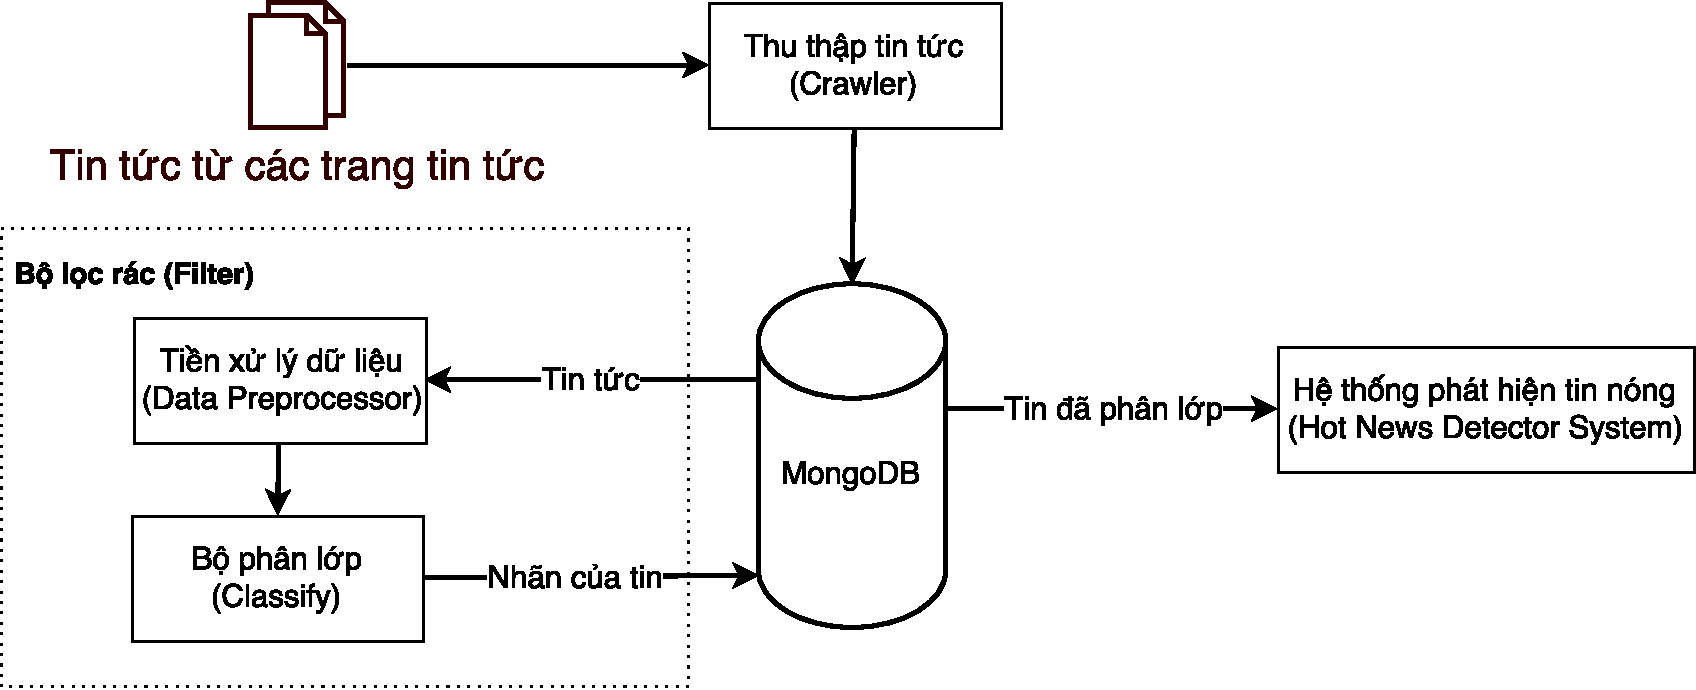
\includegraphics[width=0.9\linewidth]{Chapter3/Chapter3Figs/PDF/SystemArchitecture}
	\caption{Các thành phần chính của hệ thống}
	\label{fig:systemarchitecture}
\end{figure}

Hệ thống có 2 loại người dùng chính: quản trị viên hệ thống (admin) và biên tập viên. Quản trị viên có nhiệm vụ theo dõi hệ thống, điều khiển bật tắt, thay đổi thông số của các tác vụ trong hệ thống. Biên tập viên sử dụng hệ thống thông qua giao diện Spam Filtering để xem các sự kiện phát hiện được và các thông tin liên quan.
%\begin{itemize}
%	\item \textit{Data Streaming}: Module này sử dụng Twitter Streaming API để thu thập các bài đăng từ Twitter, theo một danh sách các từ khóa cho trước.
%	\item \textit{Data Preprocessor}: Module tiền xử lý (loại bỏ link, stopwords; tách từ) và biểu diễn dữ liệu thành vector trọng số tf-idf.
%	\item \textit{Clustering Algorithm}: Chạy thuật toán gom cụm trên dữ liệu đã mã hóa thành vector trọng số, đưa ra các cụm bài viết tương ứng và lưu vào cơ sở dữ liệu.
%	\item \textit{MongoDB}: Cơ sở dữ liệu chứa bài viết và các thông tin đính kèm, sử dụng MongoDB.
%	\item \textit{Top Stories}: Giao diện hiển thị các cụm tin tức đáng chú ý cho người dùng.
%\end{itemize}

\section{Phân hệ thu thập dữ liệu (Data Streaming)}
Module này sử dụng hệ thống Crawler để lấy các bài đăng từ nhiều nguồn tin tức lưu trữ ở cơ sở dữ liệu MySQL và đưa qua cơ sở dữ liệu MongoDB, hệ thống sẽ thực hiện các chức năng:
	\begin{itemize}
		\item Connect vào cơ sở dữ liệu mySQL để lấy các bài bài báo.
		\item Xóa các bài viết trùng.
		\item Lưu trữ xuống cơ sở dữ liệu MongoDB
	\end{itemize}
\section{Phân hệ tiền xử lý dữ liệu (Data Preprocessor)}
Module tiền xử lý có nhiệm vụ chính gồm loại bỏ URL, thực hiện tách từ, loại bỏ stopwords và biểu diễn dữ liệu thành vector trọng số tf-idf. Trước khi chạy thuật toán phân loại, dữ liệu được lấy ra từ MongoDB và tiền xử lý phần nội dung của bài báo bằng các bước sau:
	\begin{enumerate}
		\item Loại bỏ URL bằng regular expression.
		\item Tách từ sử dụng thư viện TPSegmenter. Bước này dùng để biểu diễn các từ ghép trong tiếng Việt bằng cách thêm gạch nối giữa các tiếng của từ.\\
		Ví dụ: \textit{"Vụ tai nạn 13 người chết: Đã giám định mẫu máu tài xế xe tải"} qua bộ tách từ sẽ thành \textit{"Vụ tai\_nạn 13 người chết : Đã giám\_định mẫu máu tài\_xế xe\_tải"}.
		\item Loại bỏ các từ trong danh sách gồm 813 stopwords.
		\item Tính và biểu diễn dữ liệu thành vector tf-idf và metadata.
	\end{enumerate}

\section{Phân hệ phân loại tin tức}
Sử dụng model đã train trước đó để phân loại tin tức. Model sử dụng thuật toán SVM đã trình bày ở chương 2 làm thuật toán chính để phân loại tin tức. Hiện tại hệ thống có 2 nhãn đã được định nghĩa trước đó:
	\begin{itemize}
		\item \textit Không rác
		\item \textit Rác
	\end{itemize}

Sau khi đã phân loại, hệ thống sẽ lưu nhãn đã gán cho tin tức xuống cơ sở dữ liệu MongoDB.

\section{Phân hệ phân loại loại rác}
Hệ thống sẽ lấy những tin được gán nhãn "Rác" ở bước phân loại tin tức ở trên để phân loại loại rác cho tin đó. Hiện tại có 3 loại rác đã được định nghĩa trước:
\begin{itemize}
	\item \textit Quảng cáo
	\item \textit Tuyển dụng
	\item \textit Chia sẻ
\end{itemize}

\section{Thiết kế hệ thống} 

	\begin{figure}[H]
		\centering
		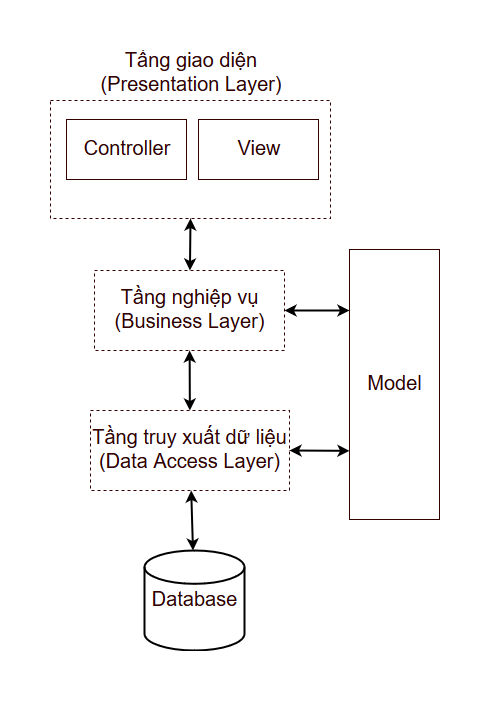
\includegraphics[width=0.5\linewidth]{Chapter3/Chapter3Figs/Layers}
		\caption{Kiến trúc hệ thống kết hợp Multilayer architecture kết hợp với mô hình MVC}
		\label{fig:layers}
	\end{figure}
Hệ thống xây dựng theo kiến trúc 3 tầng gồm: Presentation Layer, Business Logic Layer và Data Access Layer. Trong đó, Presentation Layer áp dụng mô hình Model - View - Controller (MVC). Cụ thể:
	\begin{itemize}
		\item Presentation Layer: Có trách nhiệm hiển thị thông tin, tương tác với người dùng hệ thống. Gồm 2 thành phần:
			\begin{itemize}
				\item Controller: Điều khiển các luồng của hệ thống web, nhận các tín hiệu từ người dùng và xử lý tương ứng.
				\item View: Có nhiệm vụ hiển thị các giao diện hệ thống cho người dùng.
			\end{itemize}
		\item Model: Đối tượng chứa dữ liệu để xử lý và hiển thị.
		\item Business Layer: Chứa các nghiệp vụ của hệ thống. Bao gồm các bước xử lý dữ liệu, thuật toán gom cụm, các tác vụ thống kê,...
		\item Data Access Layer: Có nhiệm vụ giao tiếp với các hệ cơ sở dữ liệu.
	\end{itemize}

\section{Cài đặt hệ thống}%các packages
Hệ thống ứng dụng được xây dựng trên nền tảng Java EE với các thành phần sau:
	\begin{itemize}
		\item Ngôn ngữ: Java, HTML, CSS, JavaScript, React.
		\item Hệ cơ sở dữ liệu: MongoDB và MySQL.
		\item Thư viện, framework: Apache Struts 2, Apache Lucene, TPSegmenter, Weka
		\item Server: Apache Tomcat
	\end{itemize}

	\subsection{Các package}
	Source code chương trình được tổ chức thành các package như sau:
	\begin{itemize}
		\item vn.vccorp.crawler.bo: Chứa các business object của hệ thống
		\item vn.vccorp.crawler.config: Các file config cho hệ thống
		\item vn.vccorp.crawler.constant: Các file constant của hệ thống
		\item vn.vccorp.crawler.dao: Data Access Object, thực hiện các tác vụ đọc, ghi database
		\item vn.vccorp.crawler.dbconnection: Cung cấp kết nối đến database
		\item vn.vccorp.crawler.dto: Data Transfer Object, các đối tượng để vận chuyển dữ liệu từ database
		\item vn.vccorp.crawler.main: Các lớp bao đóng để tạo thread chạy song song các tác vụ
		\item vn.vccorp.crawler.thread: Các lớp bao đóng để tạo thread chạy song song các tác vụ
		\item vn.vccorp.crawler.util: Các công cụ hỗ trợ trong hệ thống
		
	\end{itemize}
	
	\subsection{Cơ sở dữ liệu MongoDB}
	Hệ thống sử dụng MongoDB để lưu trữ dữ liệu tin tức và quản lý kết quả gom cụm. Đây là một hệ cơ sở dữ liệu NoSQL, cung cấp khả năng mở rộng, sao lưu, phân mảnh dữ liệu tốt, và có thể thay đổi cấu trúc dữ liệu một cách linh hoạt.
	
	Dưới đây là bảng so sánh một số thuật ngữ cơ bản giữa các cơ sở dữ liệu SQL truyền thống và MongoDB:
	\begin{table}[H]
		\centering
		\setlength\extrarowheight{3pt}
		\begin{tabular}{|l|l|}
			\hline
			\textbf{Thuật ngữ SQL}	& \textbf{Thuật ngữ MongoDB}  \\\hline
			database	& database \\\hline
			table		& collection \\\hline
			row			& document hoặc BSON document \\\hline
			column		& field \\\hline
			index		& index \\\hline
			table joins	& \$lookup, embedded documents \\\hline
		\end{tabular}
		\caption{So sánh các thuật ngữ giữa SQL và MongoDB}
		\label{tab:table_3_1}
	\end{table}
	
		\subsubsection{Collection News}
		Collection này chứa thông tin về các tin lấy từ cơ sở dữ liệu MySQL, cũng là nơi lưu trữ tất cả thông tin về tweet trong hệ thống. Khi dữ liệu được stream từ MySQL về, mỗi tin chỉ có 12 trường, các trường khác sẽ được thêm vào trong quá trình hệ thống xử lý.
		\begin{table}[H]
			%				\centering
			\setlength\extrarowheight{3pt}
			\begin{tabular}{|l|l|p{7.25cm}|}
				\hline
				\textbf{Thuộc tính}     & \textbf{Loại} & \textbf{Ý nghĩa} \\\hline
				\_id           & ObjectID       & ID trong MongoDB của document \\\hline
				Id        & Int           & ID của tin tức lấy về\\\hline
				Title         & String           & Title của tin tức\\\hline
				Content & String         & Nội dung của tin tức\\\hline
				Source   & String         & Nguồn trang báo điện tử của tin tức\\\hline
				CreateTime  & Date           & Thời gian đăng của tin\\\hline
				GetTime    & Date           & Thời gian tin tức được thu thập vào cơ sở dữ liệu MySQL\\\hline
				CollectDate    & Date           & Thời gian tweet được thu thập vào cơ sở dữ liệu MongoDB\\\hline
				Author  & String        & Người viết bài báo(nếu có)\\\hline
				Category   & Integer        & Chủ đề của bài báo\\\hline
				SpamLabel & String        & Nhãn đã gán cho tin tức\\\hline
				SpamCategory   & String         & Nhãn đã gán cho loại tin rác\\\hline
				SpamLabelFeedback      & Integer        & Feedback của nhãn đã gán cho tin tức đó\\\hline
			\end{tabular}%
			
			\caption{Các trường của collection News}
			\label{tab:table_3_2}%
		\end{table}%
		
		\subsubsection{Collection HashCode}
		Collection cluster chứa các hash code cho bài báo để kiểm tra trùng cho tin tức đó.
		\begin{table}[H]
			%				\centering
			\setlength\extrarowheight{3pt}
			\begin{tabular}{|l|l|p{9cm}|}
				\hline
				\textbf{Thuộc tính}     & \textbf{Loại} & \textbf{Ý nghĩa} \\\hline
				\_id           & ObjectID       &  ID trong MongoDB của cụm\\\hline
				HashCode      & String           & Hash code của tin tức\\\hline
			\end{tabular}%
			\caption{Các trường của collection HashCode}
			\label{tab:table_3_3}%
		\end{table}%

	\subsection{Cơ sở dữ liệu MySQL}
	MySQL được dùng để lưu trữ các dữ liệu khác của hệ thống như dữ liệu người dùng, các từ khóa dùng cho việc streaming dữ liệu Twitter,...
		\subsubsection{Bảng User}
		Bảng này dùng để quản lý danh sách người dùng hệ thống.
			\begin{table}[H]
				\centering
				\setlength\extrarowheight{3pt}
				\begin{tabular}{|l|l|l|}
					\hline
					\textbf{Thuộc tính} & \textbf{Loại} & \textbf{Ý nghĩa} \\ \hline
					ID & int(11) & ID của người dùng\\\hline
					Username & varchar(100) &  Tên tài khoản\\\hline
					Password & Long &  Mật khẩu\\\hline
					Email & varchar(100) &  Địa chỉ email người dùng\\\hline
					Fullname & varchar(100) &  Họ tên đầy đủ của người dùng\\\hline
					Phone & varchar(20) &  Số điện thoại\\\hline
					UserTypeId & int(11) &  ID phân loại người dùng\\\hline
				\end{tabular}
				\caption{Bảng User}
				\label{tab:usertable}
			\end{table}
\section{Kết quả}
Hệ thống đã hoàn thiện các chức năng: Thu thập dữ liệu từ Twitter, điều khiển chạy luồng của thuật toán phát hiện tin nóng, và hiển thị kết quả cho biên tập viên. Dưới đây là một số hình ảnh của hệ thống:

\begin{figure}[H]
	\centering
	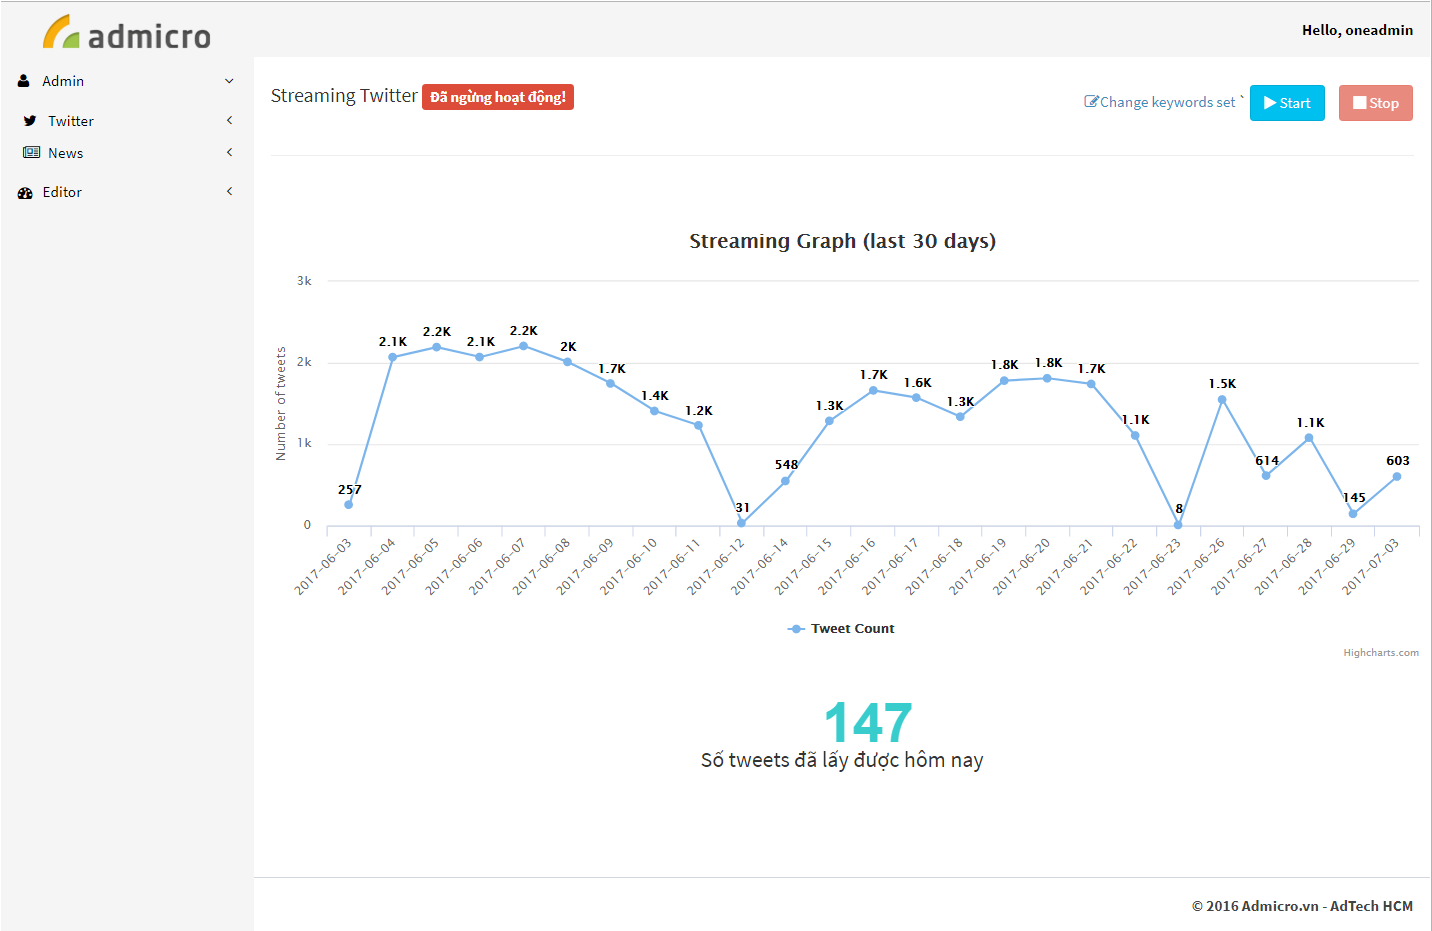
\includegraphics[width=1\linewidth]{Chapter3/Chapter3Figs/StreamingNonwide}
	\caption{Giao diện điều khiển thu thập dữ liệu Twitter}
	\label{fig:streaming}
\end{figure}

\begin{figure}[H]
	\centering
	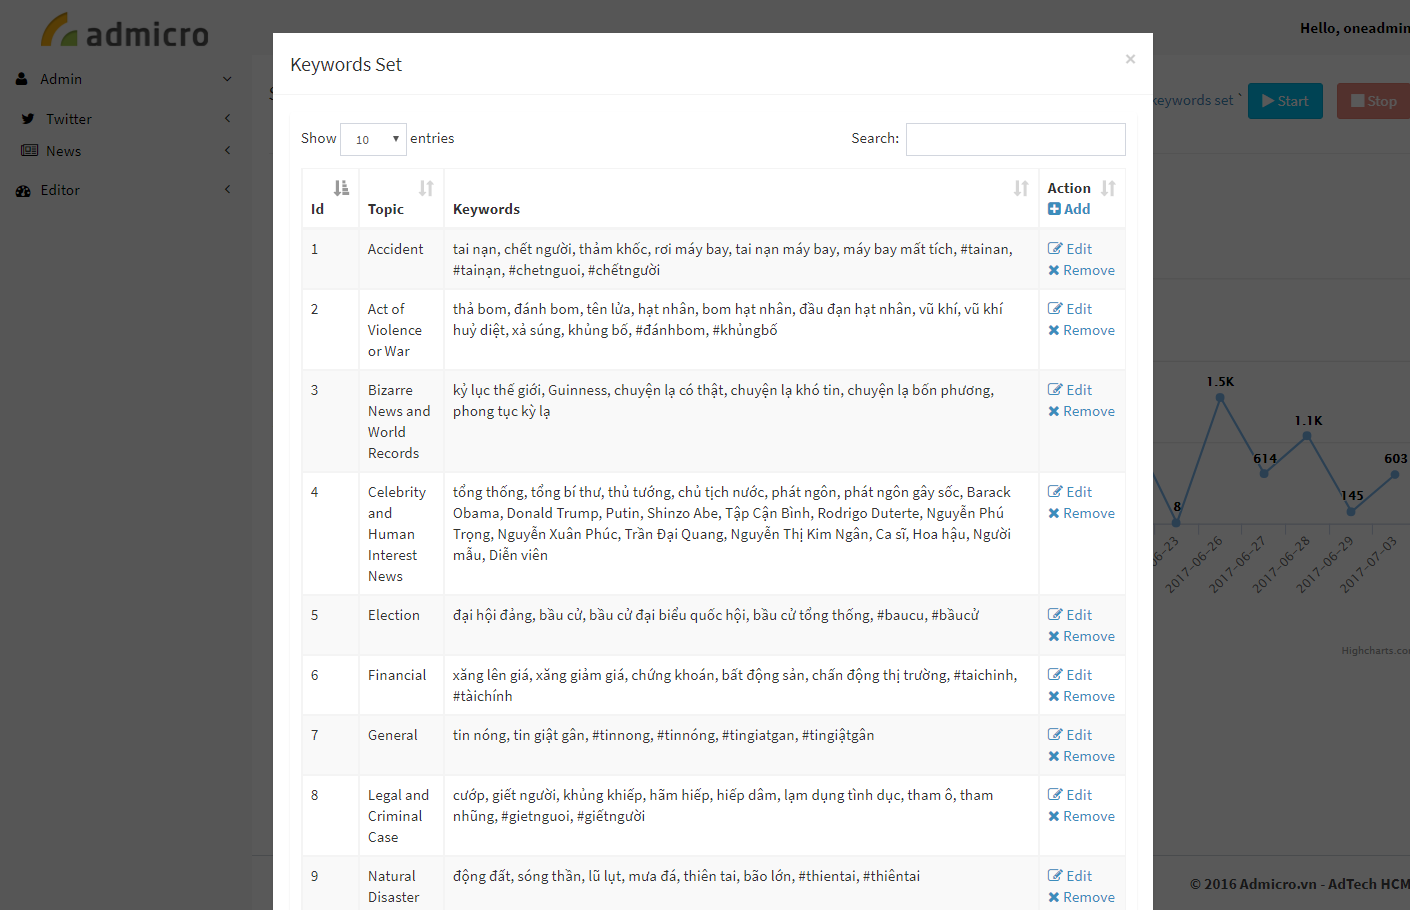
\includegraphics[width=0.96\linewidth]{Chapter3/Chapter3Figs/StreamingKeywords}
	\caption{Giao diện thêm xóa từ khóa để thu thập dữ liệu Twitter}
	\label{fig:streamingkeywords}
\end{figure}

\begin{figure}[H]
		\centering
	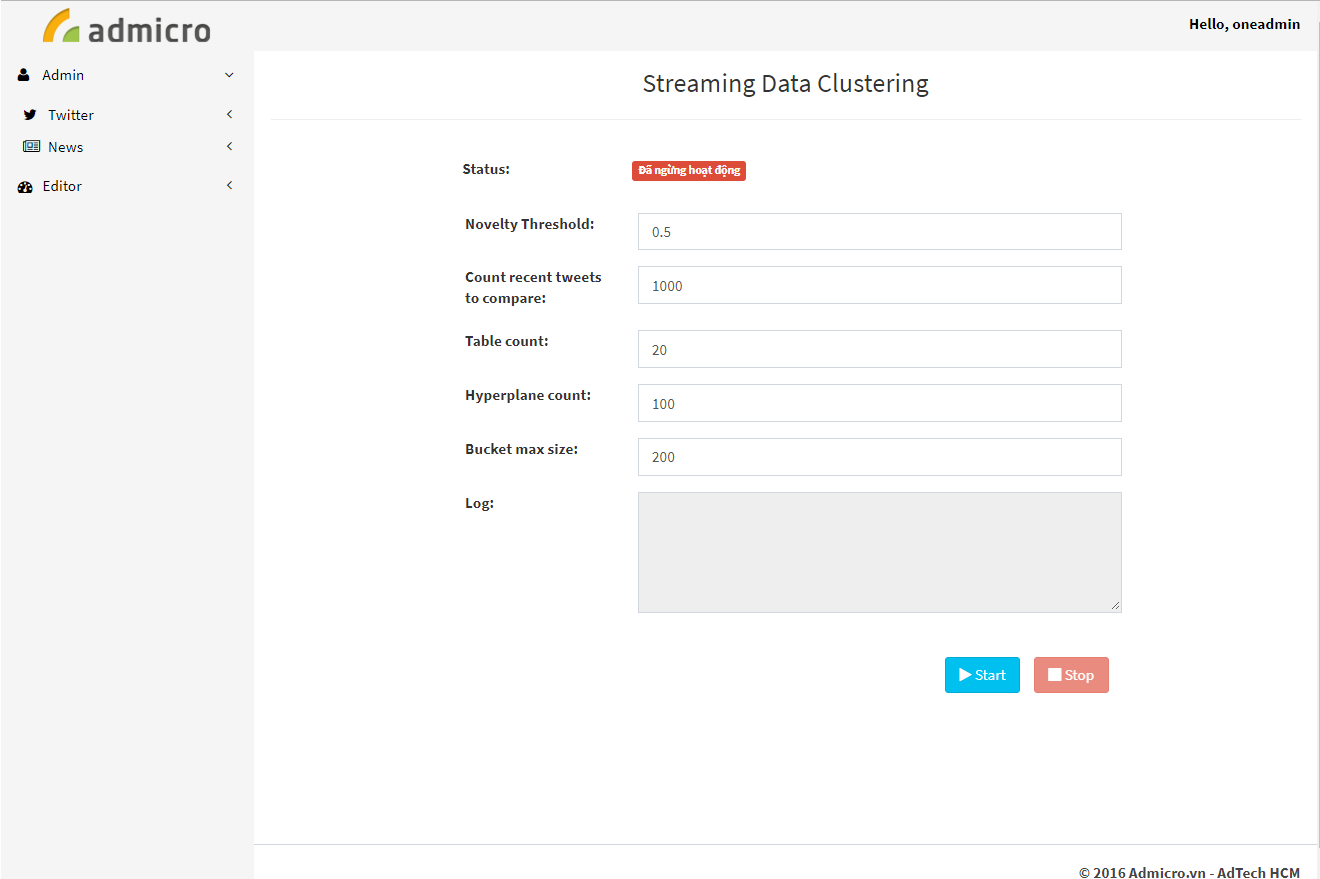
\includegraphics[width=0.96\linewidth]{Chapter3/Chapter3Figs/StartClustering}
	\caption{Giao diện điều khiển thuật toán phát hiện tin nóng}
	\label{fig:startclustering}
\end{figure}

\begin{figure}[H]
		\centering
	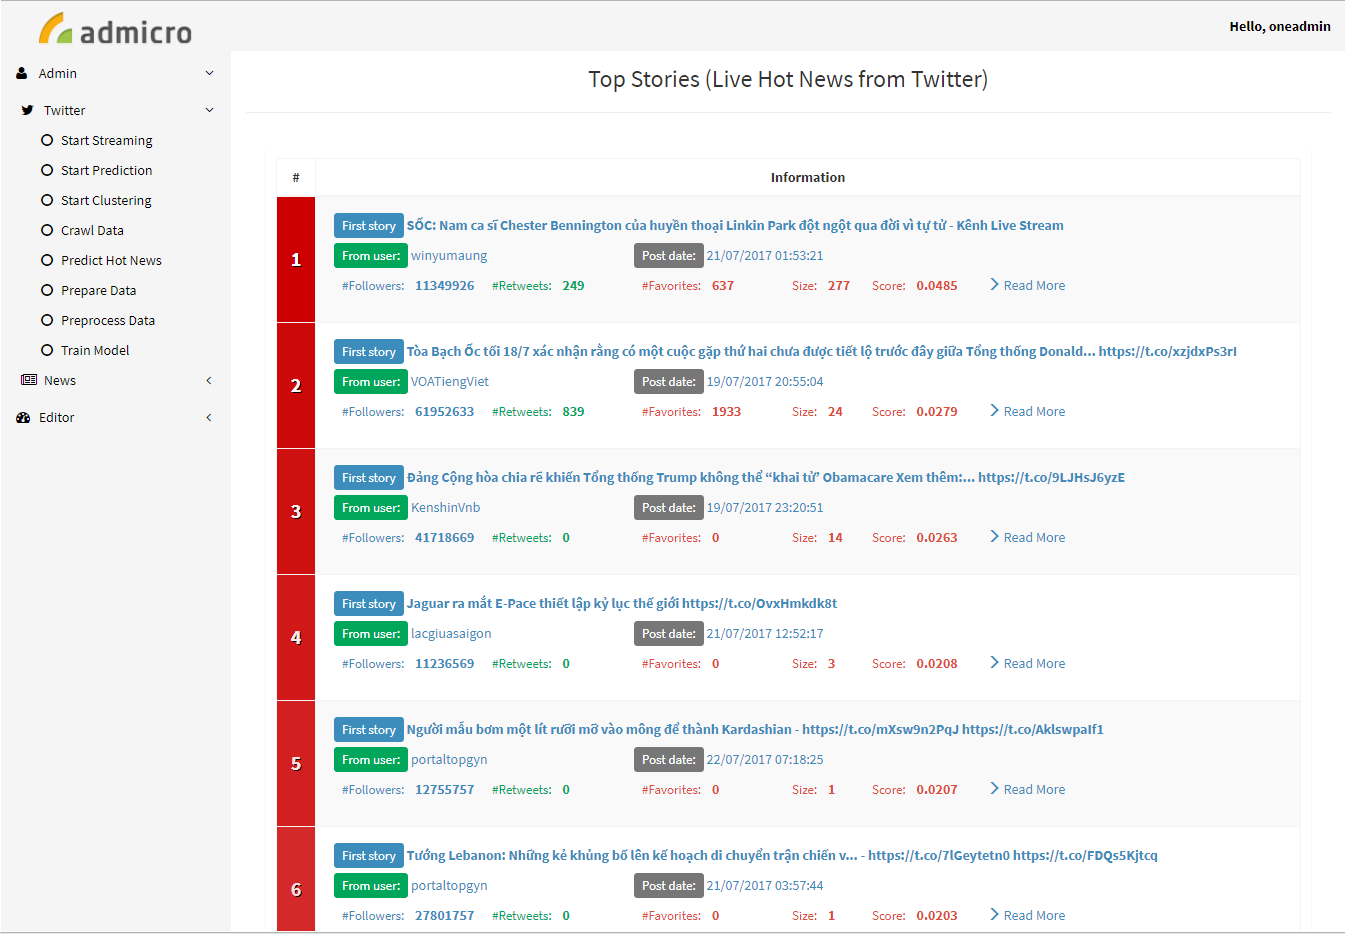
\includegraphics[width=0.96\linewidth]{Chapter3/Chapter3Figs/TopStories2}
	\caption{Giao diện hiển thị các cụm bài viết cho biên tập viên}
	\label{fig:topstories}
\end{figure}

\begin{figure}[H]
	\centering
	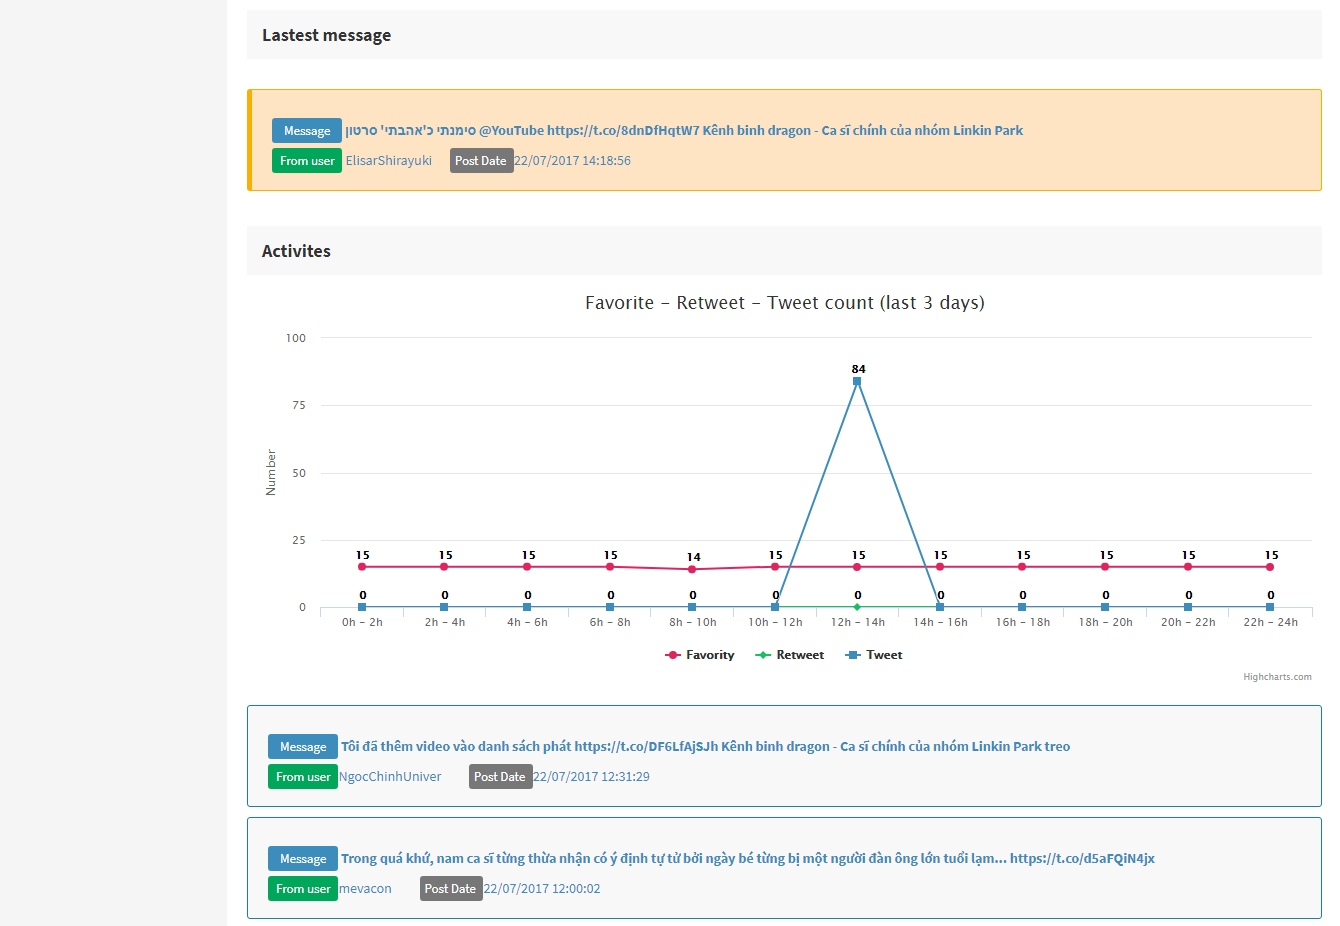
\includegraphics[width=0.96\linewidth]{Chapter3/Chapter3Figs/StoryDetails2}
	\caption{Chi tiết một cụm bài viết}
	\label{fig:storydetail}
\end{figure}

\section{Kết chương}
Chương này đã trình bày về các thành phần chính hệ thống, kiến trúc phân tầng, các hệ cơ sở dữ liệu được sử dụng và cách tổ chức, cùng một số kết quả cài đặt hệ thống.